
\subsection{Vista de proceso}

Se muestran los componentes ejecutables que funcionan en el sistema en 
tiempo de ejecución. El análisis y diseño realizado han dado lugar a 
varios componentes (SWAML, configWizard, Buxon, FOAF Enricher y 
KML Exporter) que interactuan según el diagrama de componentes descrito 
en la figura~\ref{fig:uml:componentes}.

\begin{figure}[H]
	\centering
	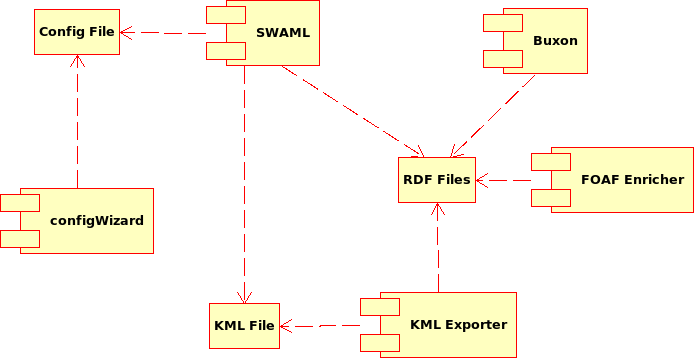
\includegraphics[width=14cm]{images/uml/componentes.png}
	\caption{Diagrama de componentes}
	\label{fig:uml:componentes}
\end{figure}

\subsubsection{SWAML}

Representa el núcleo principal de la aplicación, formado por el script
\texttt{swaml.py}. Implementa toda la lógica de la aplicación para
exportar un mailbox a RDF.

\subsubsection{configWizard}

Mediante el script \texttt{configWizard.py} se provee una forma ágil y 
sencilla de crear los ficheros de configuración que debe recibir SWAML 
como entrada.

\subsubsection{FOAF Enricher}

Representa el medio para enriquecer la información de los suscriptores
usando sus ficheros FOAF con fuente primaria de información.

\subsubsection{KML Exporter}

Mediante este componente se obtiene la información geográfica de los
distintos suscriptores de una lista de correo.

\subsubsection{Buxon}

Representa la interfaz de usuario para visualizar listas de correo
exportadas en SIOC.



